\def\fileversion{v1.0} \def\filedate{2018/07/20}
%% Package and Class "uiucthesis2009" for use with LaTeX2e.
\documentclass[edeposit,fullpage]{uiucthesis2009}
\usepackage[acronym,toc]{glossaries}
\usepackage{graphicx}
%\newacronym{<++>}{<++>}{<++>}
%\newacronym{<++>}{<++>}{<++>}

\newacronym{MTHM}{MTHM}{metric ton of heavy metal}
\newacronym{XS}{XS}{cross-sections}
\newacronym{AO}{AO}{Axial Offset}
\newacronym{PCI}{PCI}{Pellet-Cladding Interaction}
\newacronym{PCMI}{PCMI}{Pellet-Cladding Material Interaction}
\newacronym{lhr}{LHR}{Linear Hear Rate}
\newacronym{SCC}{SCC}{Stress Corrosion Cracking}
\newacronym{MPS}{MPS}{Missing Pellet Surface}

\newacronym{BOC}{BOC}{Beginning of Cycle}
\newacronym{BOL}{BOL}{Beginning of Life}
\newacronym{HZP}{HZP}{Hot Zero Power}
\newacronym{HFP}{HFP}{Hot Full Power}
\newacronym{CASL}{CASL}{Consortium for Advanced Simulation of Light Water Reactors}
\newacronym{IFBA}{IFBA}{Integral Fuel Burnable Absorber}
\newacronym{UMich}{UMich}{University of Michigan}
\newacronym{NCSU}{NCSU}{North Carolina State University}
\newacronym{ORNL}{ORNL}{Oak Ridge National Laboratory}
\newacronym{CMFD}{CMFD}{Coarse Mesh Finite Diference}
\newacronym{INL}{INL}{Idaho National Laboratory}
\newacronym{MOOSE}{MOOSE}{Multiphysics Object Oriented Simulation Environment }
\newacronym{ITC}{ITC}{Isothermal Temperature Coefficient }
\newacronym{CRW}{CRW}{Control Rod Worth}




\newacronym{DOE}{DOE}{Department of Energy}
\newacronym{EPA}{EPA}{Environmental Protection Agency}
\newacronym{EFPD}{EFPD}{Effective Full Power Days}
\newacronym{EOC}{EOC}{End of Cycle}
\newacronym{GWDMT}{GWDMT}{GigaWatt Day per Metric Ton}
\newacronym{DRWM}{DRWM}{Dynamic Rod Worth Measurement}


\newacronym{LWR}{LWR}{Light Water Reactor}
\newacronym{LPPT}{LPPT}{Low Power Physics Tests}

\newacronym{MIT}{MIT}{the Massachusetts Institute of Technology}


\newacronym{NEUP}{NEUP}{Nuclear Energy University Programs}
\newacronym{NPRE}{NPRE}{Department of Nuclear, Plasma, and Radiological Engineering}
\newacronym{NRC}{NRC}{Nuclear Regulatory Commission}

\newacronym{PARCS}{PARCS}{Purdue Advanced Reactor Core Simulator}
\newacronym{PATHS}{PATHS}{PARCS Advanced Thermal Hydraulic Solver}
\newacronym{PWR}{PWR}{Pressurized Water Reactor}
\newacronym{BWR}{BWR}{Boiling Water Reactor}

\newacronym{UOX}{UOX}{uranium oxide}
\newacronym{UQ}{UQ}{uncertainty quantification}
\newacronym{US}{U.S.}{United States}
\newacronym{UIUC}{UIUC}{University of Illinois at Urbana-Champaign}
\newacronym{VV}{V\&V}{verification and validation}
\newacronym{VERA}{VERA}{Virtual Enviromnment for Reactor Analysis}
\newacronym{VERACS}{VERA-CS}{VERA Core Simulator}
\newacronym{BEAVRS}{BEAVRS}{Benchmark for Evaluation And Validation of Reactor Simulations}
\newacronym{BW}{B\&W-1484}{Babcock and Wilcox critical experiments Series 1484}



\begin{document}

\title{Investigation of Pellet Clad Interaction during Load-Follow\\
       Operation in a Pressurized Water Reactor using VERA-CS}
\author{Daniel John O'Grady}
\department{Nuclear, Plasma, and Radiological Engineering}
\schools{B.S., University of Illinois at Urbana-Champaign, 2017}
\msthesis
\advisor{Tomasz Kozlowski}
\degreeyear{2018}
\committee{Professor Tomasz Kozloski, Advisor}%\\Professor Katherine Huff}
\maketitle

\frontmatter

%% Create an abstract that can also be used for the ProQuest abstract.
%% Note that ProQuest truncates their abstracts at 350 words.
\begin{abstract}
This is a comprehensive study of caffeine consumption by graduate
students at the University of Illinois who are in the very final
stages of completing their doctoral degrees. A study group of six
hundred doctoral students\ldots.
\end{abstract}

%% Create a dedication in italics with no heading, centered vertically
%% on the page.
\begin{dedication}
To Father and Mother.
\end{dedication}

%% Create an Acknowledgements page, many departments require you to
%% include funding support in this.
\chapter*{Acknowledgments}

This project would not have been possible without the support of
many people. Many thanks to my adviser, Lawrence T. Strongarm, who
read my numerous revisions and helped make some sense of the
confusion. Also thanks to my committee members, Reginald Bottoms,
Karin Vegas, and Cindy Willy, who offered guidance and support.
Thanks to the University of Illinois Graduate College for awarding
me a Dissertation Completion Fellowship, providing me with the
financial means to complete this project. And finally, thanks to
my husband, parents, and numerous friends who endured this long
process with me, always offering support and love.

%% The thesis format requires the Table of Contents to come
%% before any other major sections, all of these sections after
%% the Table of Contents must be listed therein (i.e., use \chapter,
%% not \chapter*).  Common sections to have between the Table of
%% Contents and the main text are:
%%
%% List of Tables
%% List of Figures
%% List Symbols and/or Abbreviations
%% etc.

\tableofcontents
\listoftables
\listoffigures

%% Create a List of Abbreviations. The left column
%% is 1 inch wide and left-justified
\chapter{List of Abbreviations}

\begin{symbollist*}
\item[CA] Caffeine Addict.
\item[CD] Coffee Drinker.
\end{symbollist*}

%% Create a List of Symbols. The left column
%% is 0.7 inch wide and centered
\chapter{List of Symbols}

\begin{symbollist}[0.7in]
\item[$\tau$] Time taken to drink one cup of coffee.
\item[$\mu$g] Micrograms (of caffeine, generally).
\end{symbollist}

\mainmatter

%%%%%%%%%%%%%%%%%%%%%%%%%%%%%%%%%%%%%%%%%%%%%%%%%%%%%%%%%
%%%%%%%%%%%%%%%%%%%%%%%%%%%%%%%%%%%%%%%%%%%%%%%%%%%%%%%%%
\chapter{Introduction}
%%%%%%%%%%%%%%%%%%%%%%%%%%%%%%%%%%%%%%%%%%%%%%%%%%%%%%%%%
%%%%%%%%%%%%%%%%%%%%%%%%%%%%%%%%%%%%%%%%%%%%%%%%%%%%%%%%%

In the \gls{US}, nuclear power generation has high fixed costs and low variable costs. 
As a result, utilities have traditionally sought to operate nuclear stations at full power from \gls{BOC} to \gls{EOC}. 
More recently, the deregulation of the energy market and the emergence of intermittent renewable energy sources have caused load-follow operation to become a more attractive option for nuclear generation. 

The deregulation of the energy market has forced utilities to compete against each other to sell electricity within a region.
The beneficiary of this competition are the customers, who are guaranteed fair prices for electricity and will not be footing the bill for an inefficient/uneconomical utility project. %need citation
Nuclear stations have typically been able to economically compete within deregulated markets because the typical plant lifetime of at least 20 years allows owners to spread out the fixed costs.
Recently, the low price of natural gas and government subsidized renewable energy sources, such as wind and solar, have made nuclear stations appear uneconomic.   

%%%%%%%%%%%%%%%%%%%%%%%%%%%%%%%%%%%%%%%%%%%%%%%%%%%%%%%%%
\section{Background and Motivation}
%%%%%%%%%%%%%%%%%%%%%%%%%%%%%%%%%%%%%%%%%%%%%%%%%%%%%%%%%

In 2016, the \gls{US} had approximately 7\% of its total electricity generation coming from wind and solar power \cite{u.s_energy_information_administration_electricity_2016}. 
This share is likely to increase as the \gls{US} continues to move away from fossil fuels and towards a "greener" energy future.
As a result of this increase, in combination with the deregulation of the energy market, the price of electricity has become volatile. 
At certain times, the price of selling electricity within a region can even become negative, due a sudden increase in renewable energy output and a low market demand \cite{paraschiv_impact_2014}. 
In some areas, negative electricity prices are further increased due to the fact that large generating facilities would rather sell at a loss to avoid decreasing their power level. 
This preference is caused by the high capital cost and relatively low variable costs of large generating facilities \cite{lokhov_load-following_2011}.

Nuclear stations are typically one of these large generating facilities.
As a result of the large construction costs and the fixed number of staff members that must be on site at all times, most utilities prefer to keep a reactor at full power, as it is easiest to maintain constant power. 
If instead of remaining at full power, a nuclear station operated in load-following mode, could this increase the efficiency of the plant?
During load-follow operation, a nuclear station will vary its power output in response to the anticipated demand to better suit the market needs, stabilizing the price of electricity.
Theoretically, the current operating plants were all designed with the maneuverability to respond to such change in demand \cite{lokhov_technical_2011}.
In fact, many of the reactors in France already participate in load-following maneuvers with the help of grey control rods \cite{lokhov_technical_2011}.
Grey control rods are similar to standard \gls{PWR} control rods but have significantly less rod worth \cite{yousefpour_improvement_2000}.
The low rod worth allows them to be used for reactivity control without putting significant stress on the surrounding fuel. 
In the \gls{US}, grey rods are not present in \gls{PWR}, increasing the complexity of load-follow operation \cite{lokhov_technical_2011}.
  
To participate in load-follow operation in the \gls{US}, a \gls{PWR} can use the critical boron concentration to modify the power level while making minor control rod insertion to manage the core \gls{AO} \cite{lokhov_technical_2011}.  
This practice, in addition to the response of the local Xenon concentrations, can lead to significant changes in local pin powers throughout the core.
Changes in local power can cause fuel to swell or contract, due to thermal expansion \cite{gartner_power_1984}. %need citation
If a utility chooses to ramp down the reactor during times of low demand, or high supply, the fuel pellets will contract.
When the decision is made to return the reactor back to full power, the rate at which the power can be increased is limited by the thermal expansion of the fuel pellets \cite{gartner_power_1984}.
A sudden expansion of the fuel pellet has the potential to exert additional stress on the cladding, commonly referred to as \gls{PCMI}.
\gls{PCMI} can lead to fuel failure by \gls{PCI}, and has been extensively investigated since the early 1970s.

\gls{PCI} induced fuel failure is the result of \gls{PCMI} and environmental contributions.
\gls{PCMI} is best described as the material interaction at the pellet-clad interface which creates a stress state on the fuel cladding \cite{kennard_pci_2016}.
This material interaction is commonly caused by the thermal expansion of $UO_2$ fuel pellets during changes in power.
%Oguma \cite{oguma_cracking_1983} found that a fuel pellets radius changes exponentially with its \gls{lhr}, thus large changes in power cause the fuel pellet to contact and strain the cladding.
In addition to the mechanical stress being exerted on the cladding, environmental contributions, chemical or geometrical in nature, have an adverse effect on the claddings integrity.
Chemical environments arise from the release of fission products from the fuel pellet.
Iodine and cadmium-in-cesium are considered to be the most corrosive fission products released from the pellet. %need citation
In the presence of prolonged \gls{PCMI}, the corrosive chemical environment causes inter granular crack propagation, or \gls{SCC}, through the zircaloy based cladding.
This type of cladding failure is commonly referred to as \gls{PCI}-\gls{SCC}, or "classical \gls{PCI}."

Geometric contributions to \gls{PCI} are a result of irregularities in the fuel pellet shape.
Typical \gls{LWR} fuel pellets are ceramic $UO_2$ cylinder with a height of approximately 1 cm and dishes and chamfers on the top and bottom of the pellet.
Hundreds of these pellets are stacked into a single fuel, with approximately 60,000 fuel rods in a \gls{LWR} core.
The shear quantity of fuel pellets ordered by a utility makes it impossible for a fuel vendor to ensure no pellet has a defect.
The most common defect is a \gls{MPS}, where part of the fuel pellet has chipped off during manufacturing.
This chip causes asymmetric expansion of the pellet during power maneuvers leading to an increased local stress on the fuel cladding. 
If this stress exceeds the yield stress of the cladding, brittle failure is likely to occur.
This type of cladding failure is commonly referred to as \gls{PCI}-\gls{MPS}, as the missing surface is the critical feature in causing the failure.

%%%%%%%%%%%%%%%%%%%%%%%%%%%%%%%%%%%%%%%%%%%%%%%%%%%%%%%%%
\section{Literature Review}
%%%%%%%%%%%%%%%%%%%%%%%%%%%%%%%%%%%%%%%%%%%%%%%%%%%%%%%%%

In the early 1970's a string of fuel failures in \gls{BWR} led to the first classification of \gls{PCI} induced fuel failure.  
Shortly after, \gls{PCI} induced fuel failures were found in \gls{PWR} and determined to be an inherent problem in \gls{LWR} zircaloy based fuels. %Find citation
The majority of these failures were observed during or shortly after power maneuvers from hot zero power.
To reduce the risk of failure, fuel manufactures made design modifications and began to provide power ramping guidelines \cite{kennard_pci_2016}.
These ramp guideline were particularly conservative and focused primarily on \gls{BOC} power ramps. 
Since then, \gls{PCI} has been extensively studied in order to increase the efficiency of reactor start-up and minimize the number of fuel failures.
%In order to extend the results of these studies to load follow operation, the driving forces of \gls{PCI} must be analyzed to determine their significance mid cycle power ramps.
 
%%%%%%
%First Paper
%%%%%%
Cox \cite{cox_pellet-clad_1990} performed an extensive review of the work done on zircaloy fuel failures caused by \gls{PCI} up to 1972.
He begins by outlining all of the factors that can contribute to \gls{PCI} failures.
The most significant factor in \gls{PCI} is the geometry of the fuel pellet. 
The strain on the cladding is determined by
\begin{enumerate}
\item manufactured gap size
\item shape of the fuel pellet
\item effect of the chamfers and groves.
\end{enumerate} 
In addition to manufactured defects in the fuel pellets, he highlights that ceramic $UO_2$ also experiences a number of geometric changes as a function of radiation exposure and temperature/power level.
These changes include but are not limited to fuel pellet  densification, cracking, relocation, and thermal expansion. 
Pellet cracking and relocation contribute significantly to strain experience by the cladding due to the differential movement of the pellets  relative to one another.
This differential movement is further intensified  by the locking of crack edges into cracks with the cladding and the local coefficient of friction between the pellet/cladding.
At high exposure the coefficient of friction can approach infinity as fission products have escaped the fuel pellet and have cemented the pellet to the cladding. 

In addition to the contribution the fuel pellet geometry has on the local strain, the cladding material and geometry determine how the cladding will respond to the strain.
The wall thickness to diameter ratio and creep rate of the cladding effect the magnitude of the initial stress and the rate at which the stress decays.
The total stress imposed on the cladding a function of maximum power, which determines the total expansion of the fuel pellet, and the change in power during a power ramp, which determines the increment in cladding strain.
Cox goes on to highlight the importance of a corrosive agent at causing \gls{PCI}, noting that Iodine and Cadmium-in-Cesium are the largest contributors to the corrosive environment at the cladding surface.
To minimize the risk of \gls{PCI}, Cox emphasized the importance of fuel conditioning or holds at intermediate power during large power ramps.
Fuel conditioning allows the cladding to relieve some of the stress experienced during the initial ramp while also influencing the chemical environment.
Together these effects reduce the propagation of cracks through the cladding surfaces.
%%%%%%

%%%%%%
%Second Paper
%%%%%%
Jernkvist \cite{jernkvist_model_1995} developed a model for predicting \gls{PCI} induced fuel failure based on crack initiation and growth.
Jernkvist model stressed three key parameters involved in \gls{PCI},
\begin{itemize} 
\item cladding stress and strain are extremely localized, 
\item fuel rod failure due to \gls{PCI} is normally a result of a sudden power increase 
\item \gls{PCI} induced failure within a reactor core shows strong variability.
\end{itemize}
Jernkvist recognized that crack propagation occurs in two stages, slow intergranular propagation followed by rapid transgranular crack growth.
Due to the presence of internal flaws within the cladding, Jernkvist neglected the intergranular process.
In order to account for the stochastic nature of \gls{PCI} in reactor cores, a probabilistic treatment of the initial crack size was used.
The crack propagation velocity was then determined by the stress, temperature, and iodine concentration at the tip of the crack.
Using a finite element solver, Jernkvist calculated the stress at the tip of the crack.
If the stress was greater than the iodine stress corrosion crack threshold, the velocity was determined using a correlation requiring the temperature and iodine concentration.
To simplify the determination of the iodine concentration, a correlation was used based on the power and fuel burnup.
It was then assumed that all of the iodine collects at the pellet-pellet interface and radial pellet cracks.

With the velocity of the crack propagation known the time to cladding failure can be calculated.
Using an artificial power history, Jernkvist provides an example where the coefficient of friction is varied for the pellet-clad interface.
At sufficiently high coefficients of friction, the local stress on the cladding is high enough to grow the crack through the cladding.
This demonstration shows the importance of accurately determining the stress within the cladding when trying to predict cladding failure.
Additionally, it highlights the need for a coupled multiphysics approach as the coefficient of friction at the pellet-clad interface is a function of temperature and burnup.
%%%%%%

%%%%%%
%Third Paper
%%%%%%
One of the computational codes that attempts to incorporate this multiphysics approach is Falcon. %Need citation
Falcon is a fully coupled, thermo-mechanical, two dimensional finite element computer code being developed by \gls{EPRI}.
Building on the material properties provided in MATPRO, Falcon has the ability to simulate $UO_2$ pellet relocation, fission gas release and zircaloy cladding thermal creep.

Falcon has been extensively benchmarked and is commonly used by contractors and utilities to mitigate the risk of \gls{PCI} induced fuel failure.
Lyon et al. \cite{lyon_pci_2009} used Falcon in order to determine a criteria for mitigating \gls{PCI} induced fuel failure during power ramps.
The authors point out that power ramp rate restrictions, which are normally set by fuel vendors, and power conditioning, the practice of taking intermediate holds at constant power, are not reliable at mitigating the risk of \gls{PCI}. 
Rather, these practices lead to restrictive constraints on plant operation.

Another criteria that is commonly suggested is the implementation of a stress based threshold.
The authors argue that stress based thresholds are unable to distinguish between failed and non failed fuel rods, leading to a conservative threshold when applied to power maneuvers.
In its place they propose a mechanistic approach that incorporates \gls{PCMI} and \gls{SCC} based cumulative damage.

%Section on calculation of CDI
%
%
%

In order to demonstrate the accuracy of a \gls{CDI} based criteria, Lyon et al. simulated 14 fuel rods from the studsvik ramp program using Falcon.
These simulations were broken into three parts, first a steady state two dimensional, R-Z, depletion simulation is performed using the power histories of each rod.
The results of these simulations are then used as the initial condition for transient R-Z simulations of the different power ramps under investigation.
Finally, an R-$\theta$ model containing discrete fuel cracks is created for the axial location which experienced the highest R-Z hoop stress.
This simulation provides the fuel pins maximum clad hoop stress and \gls{CDI} which can then be used to determine a threshold criteria.
 
\begin{figure}
\begin{tabular}{cc}
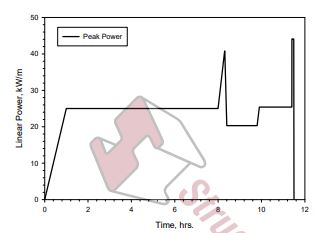
\includegraphics[width=0.5\linewidth]{./Figures/lyon_image_6.JPG} & 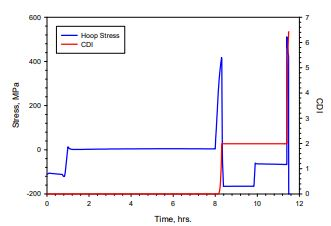
\includegraphics[width=0.5\linewidth]{./Figures/lyon_image_7.JPG}
\end{tabular}
\caption{The Power history (left), Falcon predicted hoop stress and Falcon predicted \gls{CDI} for Q11/1 of the Studsvik ramp program \cite{lyon_pci_2009}}
\label{fig:paper_3_res}
\end{figure}
%%%%%%




%%%%%%%%%%%%%%%%%%%%%%%%%%%%%%%%%%%%%%%%%%%%%%%%%%%%%%%%%
\section{Conditioned Power}
%%%%%%%%%%%%%%%%%%%%%%%%%%%%%%%%%%%%%%%%%%%%%%%%%%%%%%%%%

%%%%%%%%%%%%%%%%%%%%%%%%%%%%%%%%%%%%%%%%%%%%%%%%%%%%%%%%%
%%%%%%%%%%%%%%%%%%%%%%%%%%%%%%%%%%%%%%%%%%%%%%%%%%%%%%%%%
\chapter{PWR1}
%%%%%%%%%%%%%%%%%%%%%%%%%%%%%%%%%%%%%%%%%%%%%%%%%%%%%%%%%
%%%%%%%%%%%%%%%%%%%%%%%%%%%%%%%%%%%%%%%%%%%%%%%%%%%%%%%%%

%%%%%%%%%%%%%%%%%%%%%%%%%%%%%%%%%%%%%%%%%%%%%%%%%%%%%%%%%
\section{Plant Description}
%%%%%%%%%%%%%%%%%%%%%%%%%%%%%%%%%%%%%%%%%%%%%%%%%%%%%%%%%

%%%%%%%%%%%%%%%%%%%%%%%%%%%%%%%%%%%%%%%%%%%%%%%%%%%%%%%%%
\section{Summary of Previous Results}
%%%%%%%%%%%%%%%%%%%%%%%%%%%%%%%%%%%%%%%%%%%%%%%%%%%%%%%%%

%%%%%%%%%%%%%%%%%%%%%%%%%%%%%%%%%%%%%%%%%%%%%%%%%%%%%%%%%
\section{Load-Follow Operation}
%%%%%%%%%%%%%%%%%%%%%%%%%%%%%%%%%%%%%%%%%%%%%%%%%%%%%%%%%

%%%%%%%%%%%%%%%%%%%%%%%%%%%%%%%%%%%%%%%%%%%%%%%%%%%%%%%%%
%%%%%%%%%%%%%%%%%%%%%%%%%%%%%%%%%%%%%%%%%%%%%%%%%%%%%%%%%
\chapter{Methodology}
%%%%%%%%%%%%%%%%%%%%%%%%%%%%%%%%%%%%%%%%%%%%%%%%%%%%%%%%%
%%%%%%%%%%%%%%%%%%%%%%%%%%%%%%%%%%%%%%%%%%%%%%%%%%%%%%%%%

%%%%%%%%%%%%%%%%%%%%%%%%%%%%%%%%%%%%%%%%%%%%%%%%%%%%%%%%%
\section{BISON}
%%%%%%%%%%%%%%%%%%%%%%%%%%%%%%%%%%%%%%%%%%%%%%%%%%%%%%%%%

%%%%%%%%%%%%%%%%%%%%%%%%%%%%%%%%%%%%%%%%%%%%%%%%%%%%%%%%%
\section{MPACT Screening Process}
%%%%%%%%%%%%%%%%%%%%%%%%%%%%%%%%%%%%%%%%%%%%%%%%%%%%%%%%%

%%%%%%%%%%%%%%%%%%%%%%%%%%%%%%%%%%%%%%%%%%%%%%%%%%%%%%%%%
%%%%%%%%%%%%%%%%%%%%%%%%%%%%%%%%%%%%%%%%%%%%%%%%%%%%%%%%%
\chapter{Results and Discussion}
%%%%%%%%%%%%%%%%%%%%%%%%%%%%%%%%%%%%%%%%%%%%%%%%%%%%%%%%%
%%%%%%%%%%%%%%%%%%%%%%%%%%%%%%%%%%%%%%%%%%%%%%%%%%%%%%%%%

%%%%%%%%%%%%%%%%%%%%%%%%%%%%%%%%%%%%%%%%%%%%%%%%%%%%%%%%%
\section{BISON}
%%%%%%%%%%%%%%%%%%%%%%%%%%%%%%%%%%%%%%%%%%%%%%%%%%%%%%%%%

%%%%%%%%%%%%%%%%%%%%%%%%%%%%%%%%%%%%%%%%%%%%%%%%%%%%%%%%%
\section{Limiting Pin}
%%%%%%%%%%%%%%%%%%%%%%%%%%%%%%%%%%%%%%%%%%%%%%%%%%%%%%%%%

%%%%%%%%%%%%%%%%%%%%%%%%%%%%%%%%%%%%%%%%%%%%%%%%%%%%%%%%%
%%%%%%%%%%%%%%%%%%%%%%%%%%%%%%%%%%%%%%%%%%%%%%%%%%%%%%%%%
\chapter{Conclusions}
%%%%%%%%%%%%%%%%%%%%%%%%%%%%%%%%%%%%%%%%%%%%%%%%%%%%%%%%%
%%%%%%%%%%%%%%%%%%%%%%%%%%%%%%%%%%%%%%%%%%%%%%%%%%%%%%%%%

We conclude that graduate students like coffee.

\backmatter
\bibliographystyle{ans}
\bibliography{Masters}

\chapter{Vita}

Juan Valdez was born\ldots.

\end{document}
\endinput
%%
%% End of file `thesis-ex.tex'.
